\documentclass[11pt,letterpaper]{article}

\usepackage[utf8]{inputenc}
\usepackage[T1]{fontenc}
\usepackage[spanish,es-tabla,es-nodecimaldot]{babel}
\usepackage{mathptmx}                  % Times New Roman
\usepackage[margin=2.5cm]{geometry}
\usepackage{setspace}
\usepackage{graphicx}
\usepackage{float}
\usepackage{xcolor}
\usepackage{listings}
\usepackage{booktabs}
\usepackage{caption}
\usepackage{enumitem}
\usepackage{fancyhdr}
\usepackage{pdflscape}
\usepackage[hidelinks]{hyperref}

\onehalfspacing
\setlength{\parskip}{4pt}
\captionsetup{font=small,labelfont=bf}
\setlist{itemsep=1pt,topsep=2pt}

\pagestyle{fancy}
\fancyhf{}
\fancyhead[L]{\small TC5061. Operaciones de Aprendizaje Automático (MLOps)}
\fancyhead[R]{\small A01840539}
\fancyfoot[C]{\small\thepage}
\renewcommand{\headrulewidth}{0.4pt}

% Enlaces del entregable
\newcommand{\repo}{https://github.com/neronapier/TC5061-A03-Experimentacion-MLflow}
\newcommand{\mlflowui}{https://161.132.54.170}

\definecolor{codebg}{HTML}{F7F7F9}
\lstdefinestyle{bash}{
  language=bash,
  backgroundcolor=\color{codebg},
  basicstyle=\ttfamily\footnotesize\setstretch{1.0},
  frame=single,
  rulecolor=\color{gray!40},
  breaklines=true,
  columns=fullflexible,
  keepspaces=true,
  upquote=true,
  showstringspaces=false,
}

\begin{document}
\sloppy

% ============================== PORTADA ======================================
\begin{titlepage}
\centering
\vspace*{1.2cm}


\includegraphics[width=0.52\textwidth]{logo_tec.png}\\[1.1cm]

{\large Maestría en Inteligencia Artificial Aplicada}\\[1.8cm]

\rule{\linewidth}{0.5pt}\\[0.5cm]
{\LARGE\bfseries Actividad 3\\[0.35cm]
Código de experimentación base con MLflow}\\[0.4cm]
\rule{\linewidth}{0.5pt}\\[2cm]

{\large
\begin{tabular}{rl}
\textbf{Alumno:} & Jordan Piero Borda Colque\\[0.25cm]
\textbf{Matrícula:} & A01840539\\[0.25cm]
\textbf{Correo:} & \href{mailto:A01840539@tec.mx}{A01840539@tec.mx}\\[0.25cm]
\textbf{Curso:} & TC5061: Operaciones de Aprendizaje\\
                & Automático (MLOps)\\[0.25cm]
\textbf{Profesor titular:} & Iván Reyes Amezcua\\[0.25cm]
\textbf{Fecha:} & 11 de octubre de 2026\\
\end{tabular}}

\vfill
\end{titlepage}

% ============================== 1 ============================================
\section{Repositorio y ejecución}

\begin{itemize}
  \item \textbf{Repositorio:} \url{\repo}
  \item \textbf{MLflow (solo lectura):} \url{\mlflowui}
  \item \textbf{Experimento:} \texttt{TC5061\_A03\_AdultIncome\_LogReg} (10 corridas)
\end{itemize}

El modelo base de la Actividad 2 (regresión logística sobre UCI Adult, para predecir si una persona gana más de 50K USD
al año) pasó del notebook a \texttt{train.py}. El notebook \texttt{notebooks/eda\_adult.ipynb} conserva solo la
exploración de datos. Las corridas se ejecutaron en el VPS del curso, en Docker: MLflow 3.16.1 con artefactos
en MinIO. Comandos exactos:

\begin{lstlisting}[style=bash]
pip install -r requirements.txt
python train.py                                   # valores por defecto
python train.py --C 1 --l1-ratio 0 --class-weight balanced --seed 42 --run-name 07_l2_C1_balanced
./scripts/run_experimentos.sh                     # las 10 corridas
# En el VPS (MLFLOW_TRACKING_URI=http://mlflow:5000 dentro del contenedor):
docker compose --profile run run --rm -T -w /work/actividad3 -e PY=python runner \
    bash scripts/run_experimentos.sh
\end{lstlisting}

% ============================== 2 ============================================
\section{Implementación}

\textbf{Estructura.} Cada función de \texttt{train.py} tiene una sola responsabilidad: \texttt{parse\_args},
\texttt{fijar\_semilla}, \texttt{cargar\_datos} (descarga UCI si falta), \texttt{limpiar} (decisiones de la
Actividad 2), \texttt{construir\_modelo} (\texttt{Pipeline} con preprocesamiento y clasificador),
\texttt{evaluar}, \texttt{guardar\_artefactos} y \texttt{main}, que une todo dentro de \texttt{mlflow.start\_run()}.

\textbf{Parámetros por línea de comandos} (\texttt{argparse}, con valores por defecto y ayuda en
\texttt{--help}): \texttt{--C} (1.0), \texttt{--l1-ratio} (0 = L2, 1 = L1), \texttt{--class-weight}
(\texttt{none}/\texttt{balanced}), \texttt{--min-frequency} (50), \texttt{--max-iter} (1000) y \texttt{--seed} (42),
además de \texttt{--test-size}, \texttt{--cv-folds}, \texttt{--experiment-name} y \texttt{--run-name}.

\textbf{Registro en MLflow.} \texttt{log\_param} para cada argumento, el solver y los tamaños de entrenamiento y prueba;
\texttt{log\_metric} para 7 métricas de prueba (accuracy, balanced accuracy, precision, recall, F1, ROC-AUC y PR-AUC),
la ROC-AUC de validación cruzada (media y desviación), la ROC-AUC de entrenamiento y el número de coeficientes
distintos de cero; \texttt{log\_artifact} para la matriz de confusión con la curva ROC, el reporte de
clasificación y \texttt{metrics.json}; y \texttt{mlflow.sklearn.log\_model} para el pipeline, con firma y ejemplo
de entrada.

\textbf{Reproducibilidad.} La semilla fija \texttt{random}, \texttt{numpy} y \texttt{PYTHONHASHSEED}, y se pasa
como \texttt{random\_state} a la división, a la validación cruzada y al modelo. Las versiones están fijadas en
\texttt{requirements.txt}. La corrida 10 repite la 01 con los mismos argumentos y da las mismas métricas hasta el
último decimal. Ese mismo resultado también se obtuvo en un entorno local nuevo instalado desde
\texttt{requirements.txt}.

% ============================== 3 ============================================
\section{Corridas}

\begin{table}[H]
\centering
\small
\setstretch{1.1}
\caption{Corridas del experimento (métricas en el conjunto de prueba, $n = 9\,758$).}
\label{tab:corridas}
\begin{tabular}{@{}lrrlrrrrrrr@{}}
\toprule
\textbf{Corrida} & \textbf{C} & \textbf{l1} & \textbf{class\_w} & \textbf{mf} & \textbf{seed} &
\textbf{ROC-AUC} & \textbf{F1} & \textbf{Prec.} & \textbf{Recall} & \textbf{Coef.} \\
\midrule
01 baseline        & 1     & 0   & none     & 50  & 42 & 0.9024 & 0.6592 & 0.7195 & 0.6083 & 74 \\
02 L2 fuerte       & 0.001 & 0   & none     & 50  & 42 & 0.8954 & 0.5984 & 0.7449 & 0.5000 & 74 \\
03 L2 débil        & 100   & 0   & none     & 50  & 42 & 0.9025 & 0.6582 & 0.7175 & 0.6079 & 74 \\
04 L1              & 0.01  & 1   & none     & 50  & 42 & 0.8981 & 0.6382 & 0.7205 & 0.5728 & 19 \\
05 L1 fuerte       & 0.001 & 1   & none     & 50  & 42 & 0.8909 & 0.5470 & 0.7727 & 0.4234 & 6 \\
06 Elastic Net     & 0.1   & 0.5 & none     & 50  & 42 & 0.9024 & 0.6544 & 0.7188 & 0.6006 & 50 \\
\textbf{07 balanced} & 1   & 0   & balanced & 50  & 42 & 0.9023 & \textbf{0.6715} & 0.5572 & \textbf{0.8450} & 74 \\
08 min\_freq 500   & 1     & 0   & none     & 500 & 42 & 0.9023 & 0.6583 & 0.7202 & 0.6062 & 50 \\
09 otra semilla    & 1     & 0   & none     & 50  & 7  & 0.8993 & 0.6383 & 0.7140 & 0.5771 & 72 \\
10 repetición      & 1     & 0   & none     & 50  & 42 & 0.9024 & 0.6592 & 0.7195 & 0.6083 & 74 \\
\bottomrule
\end{tabular}
\end{table}

% ============================== 4 ============================================
\section{Análisis de resultados}

\textbf{Mejor configuración.} En ROC-AUC, que no depende del umbral, hay un empate: las corridas 01, 03, 06, 07 y 08
quedan entre 0.9023 y 0.9025. Esa diferencia es menor que la desviación estándar de la validación cruzada (0.004).
Por eso elijo la \textbf{07 (L2, $C=1$, \texttt{class\_weight=balanced})}: con la misma ROC-AUC obtiene el mejor F1
(0.672) y la mejor balanced accuracy (0.817), y sube el recall de la clase \texttt{>50K} de 0.61 a 0.85. Su costo es
menos precisión (0.56) y menos accuracy (0.80), porque predice \texttt{>50K} con más frecuencia.

\textbf{Hiperparámetro más influyente.} \texttt{class\_weight} es el que más cambia las métricas que dependen del
umbral: mueve el recall 24 puntos sin cambiar la ROC-AUC, así que en la práctica desplaza el umbral de decisión.
\texttt{C} solo influye con regularización fuerte: con $C=0.001$ la ROC-AUC baja a 0.895 (L2) y 0.891 (L1), y el
recall cae a 0.50 y 0.42; entre $C=1$ y $C=100$ no hay diferencia. L1 sirve para simplificar el modelo: con
$C=0.01$ usa 19 de 74 coeficientes y conserva una ROC-AUC de 0.898. \texttt{min\_frequency} (de 50 a 500) quita 24
columnas y no cambia el desempeño.

\textbf{Limitaciones.}
\begin{itemize}
  \item Se usa una sola partición de prueba. Cambiar solo la semilla (corrida 09) mueve el F1 en 0.021 y la ROC-AUC
        en 0.003, más que la diferencia entre las mejores configuraciones.
  \item Las corridas se eligieron a mano (10 configuraciones). Faltan una búsqueda sistemática y el ajuste del
        umbral, que daría un efecto parecido a \texttt{balanced}.
  \item Las corridas L1 y Elastic Net usan \texttt{saga} y las L2 usan \texttt{lbfgs}, así que el solver también
        cambia entre ellas.
  \item Se probó un solo modelo lineal y no se evaluó el sesgo por \texttt{sex} y \texttt{race}, que el EDA mostró
        relevante.
\end{itemize}

% ============================== ANEXO ========================================
\appendix

\begin{landscape}
\section{Evidencias de MLflow}

Las figuras se tomaron de la interfaz pública \url{\mlflowui}, donde se pueden revisar todas las corridas.

\begin{figure}[H]
\centering
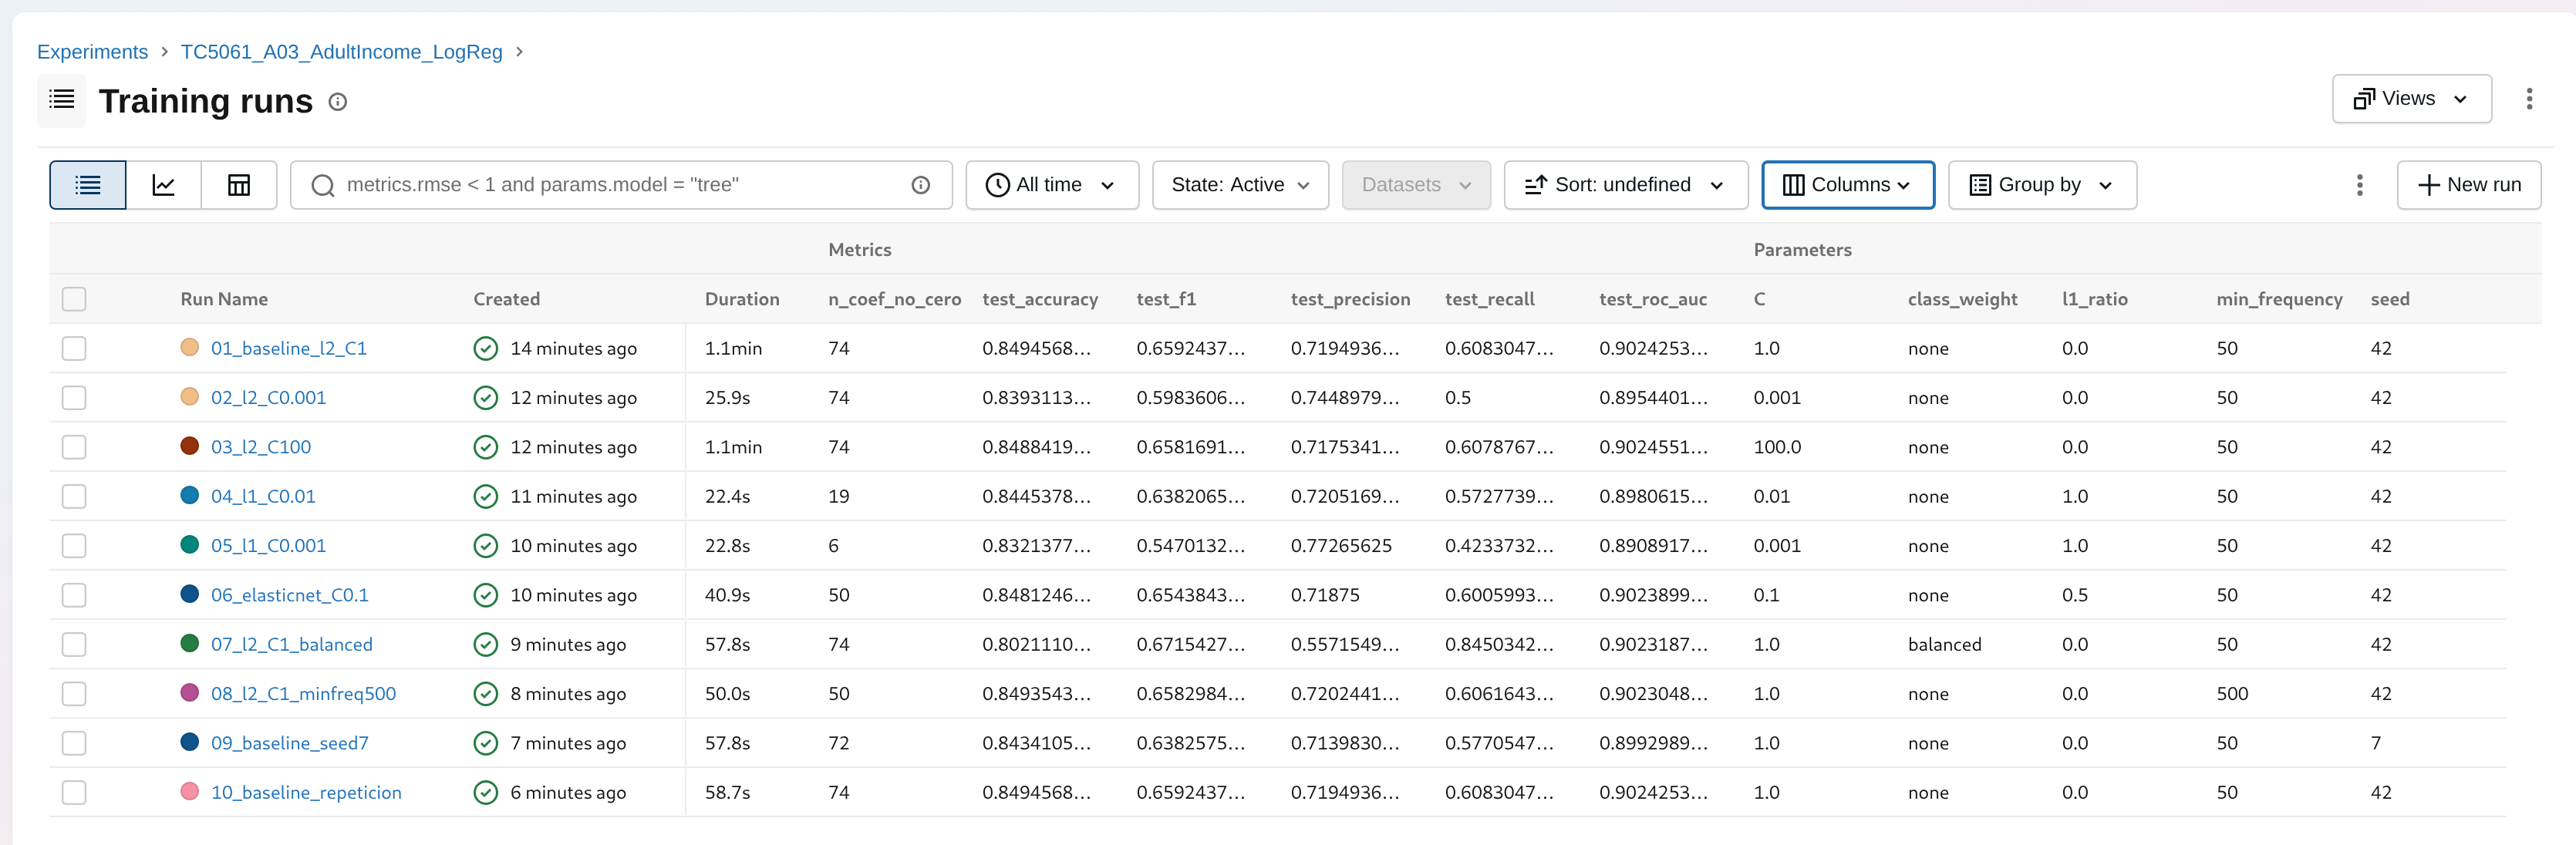
\includegraphics[width=\linewidth]{../evidencia/01_tabla_corridas.png}
\caption{Tabla comparativa de las 10 corridas en el experimento \texttt{TC5061\_A03\_AdultIncome\_LogReg}
(parámetros y métricas de prueba).}
\end{figure}
\end{landscape}

\begin{landscape}
\begin{figure}[H]
\centering
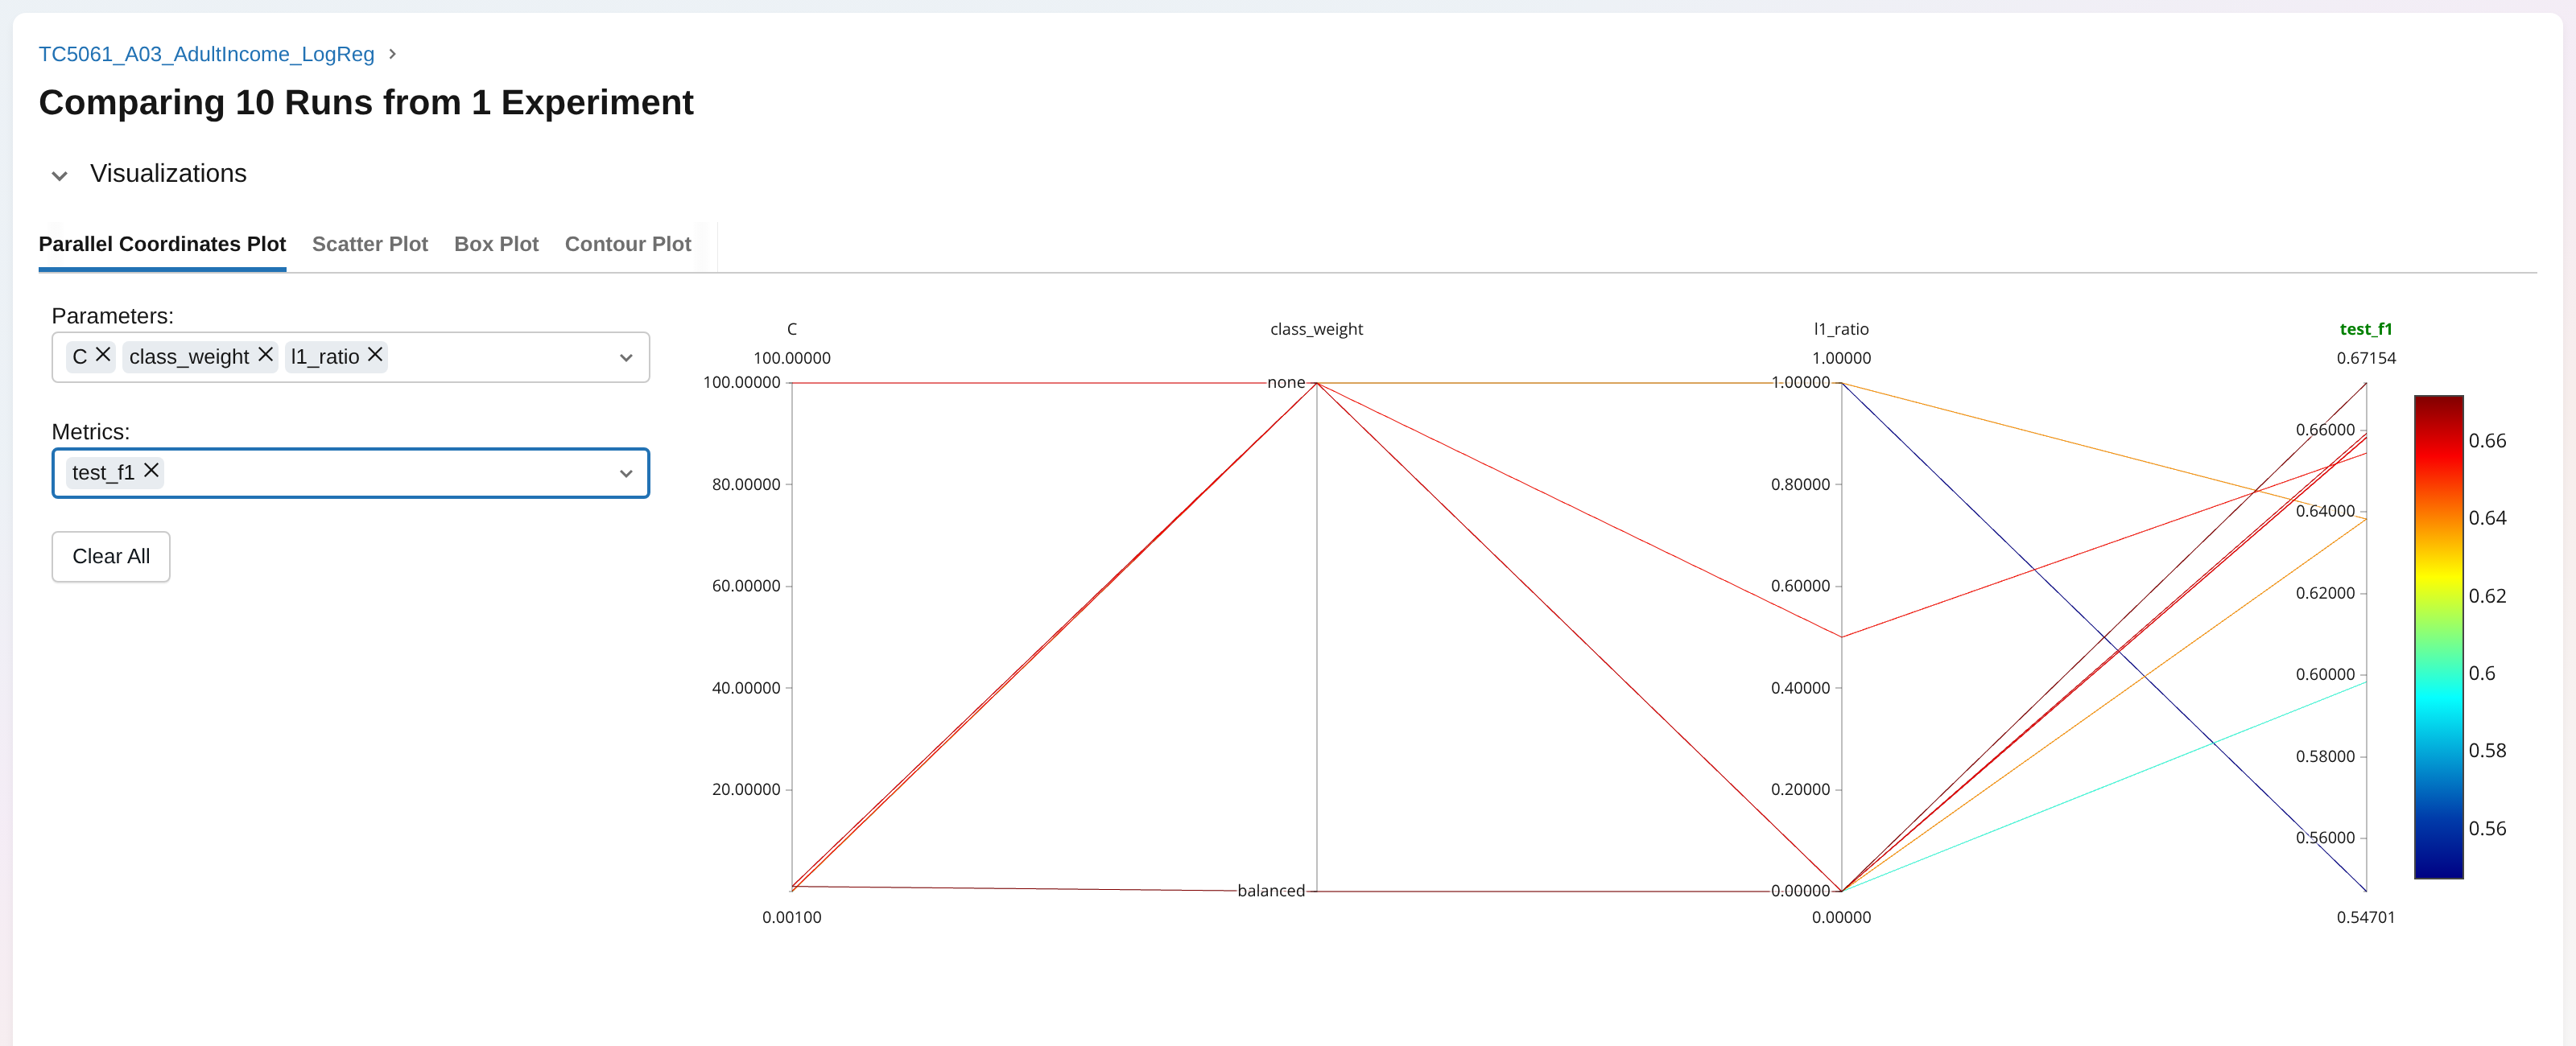
\includegraphics[width=0.92\linewidth]{../evidencia/02_comparacion_corridas.png}
\caption{Vista \textit{Compare runs}: coordenadas paralelas de \texttt{C}, \texttt{class\_weight} y
\texttt{l1\_ratio} contra \texttt{test\_f1}.}
\end{figure}
\end{landscape}

\begin{figure}[H]
\centering
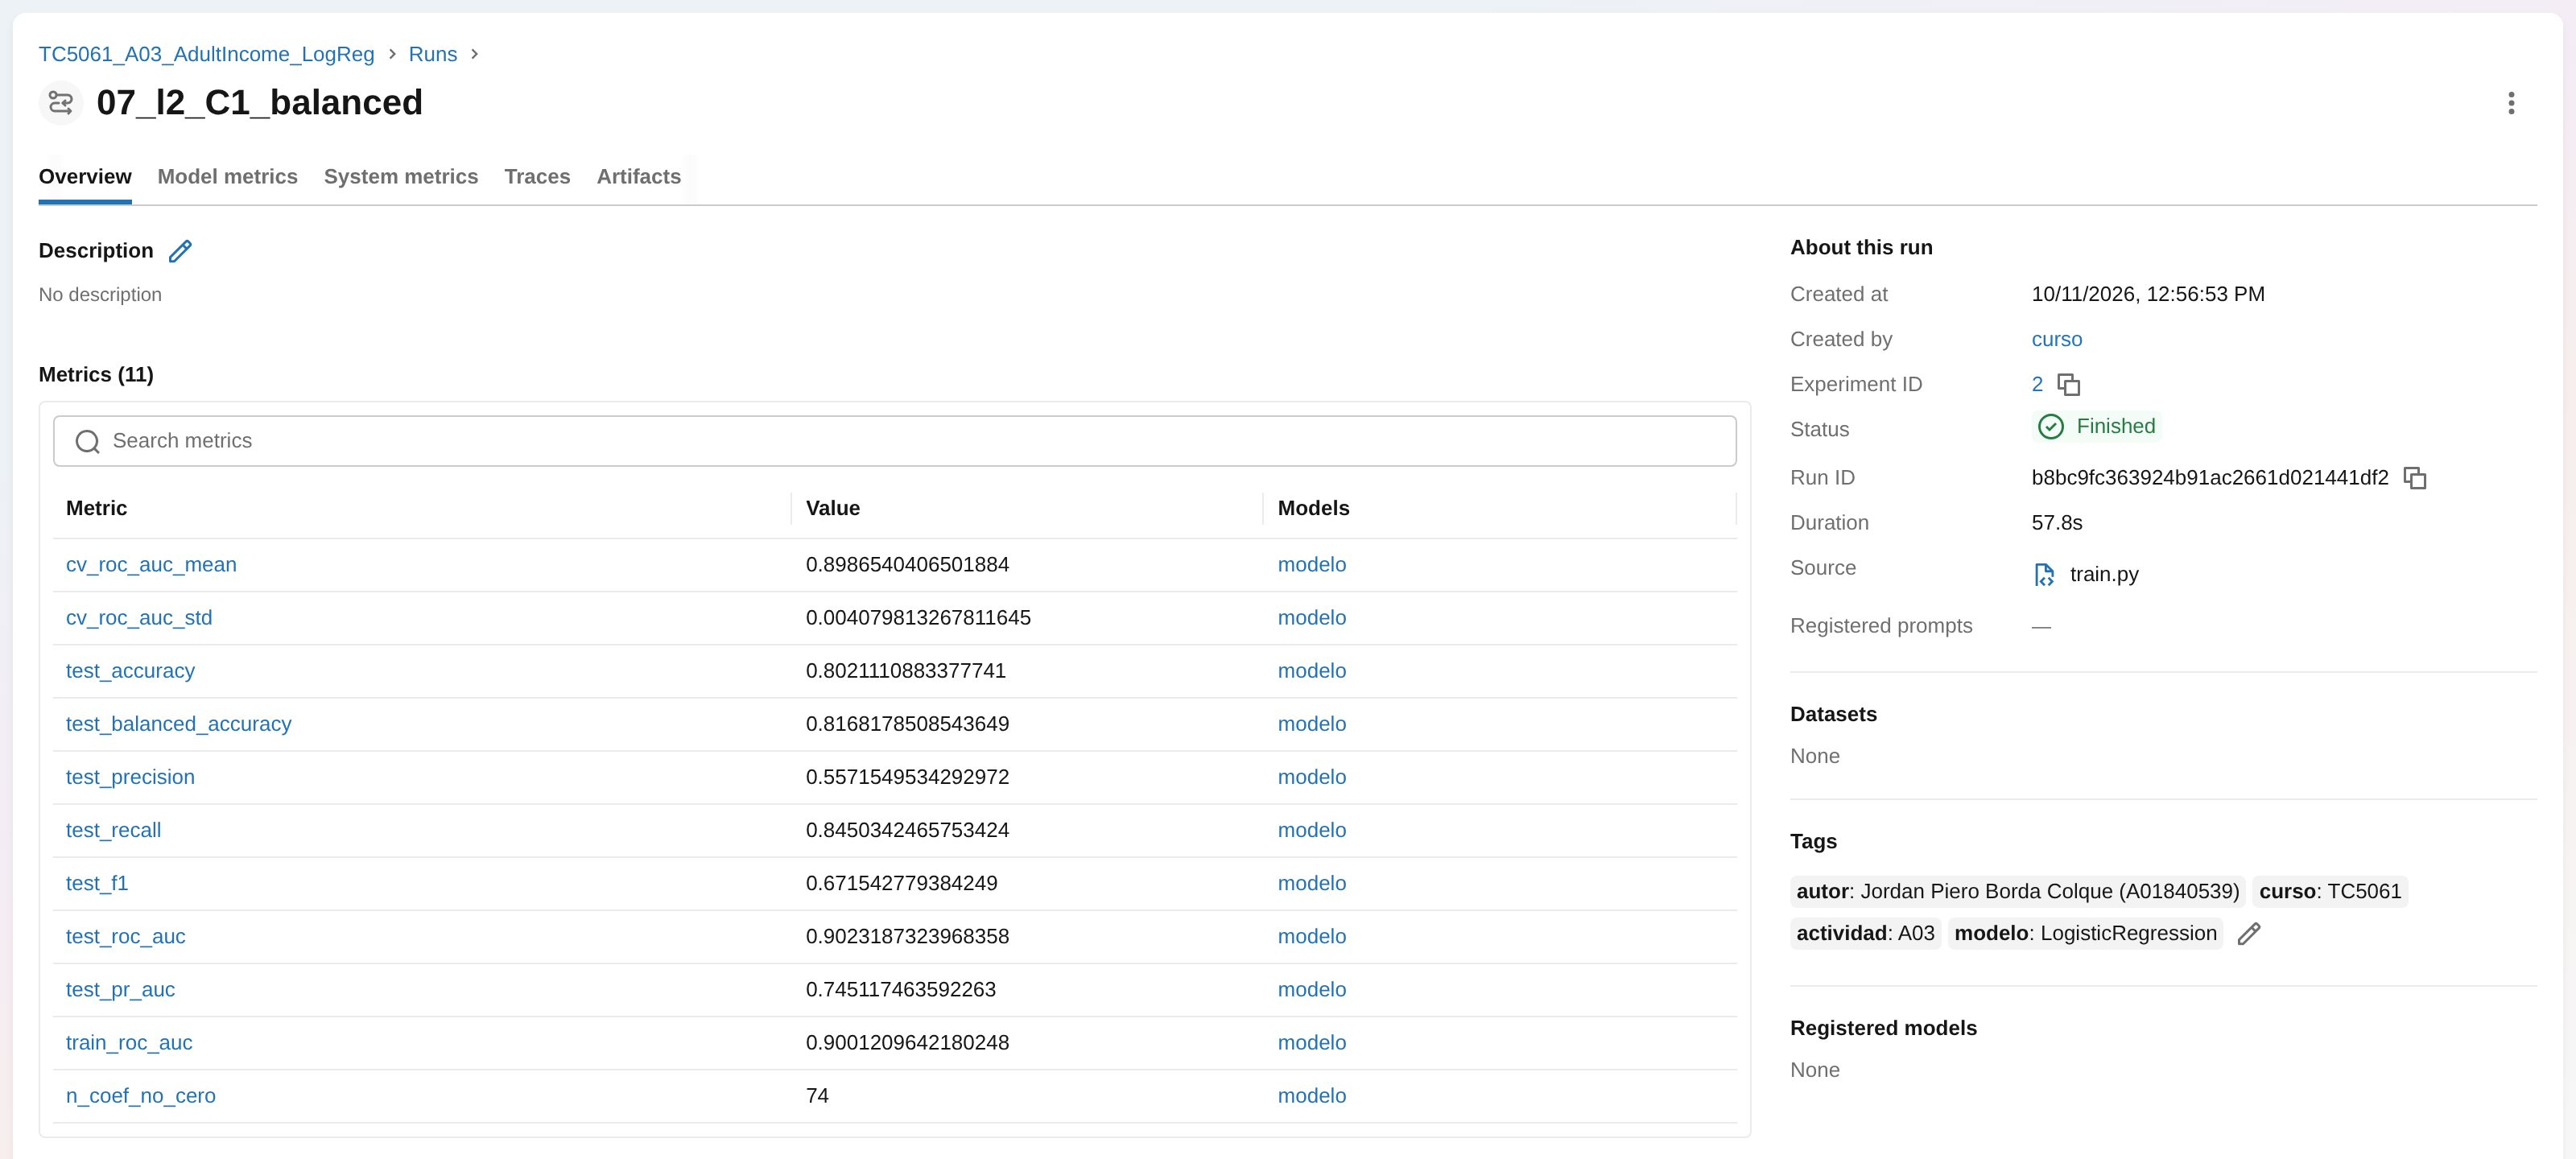
\includegraphics[width=0.9\textwidth]{../evidencia/03_corrida_detalle.png}
\caption{Detalle de la corrida \texttt{07\_l2\_C1\_balanced}: métricas, tags y modelo asociado.}
\end{figure}

\begin{figure}[H]
\centering
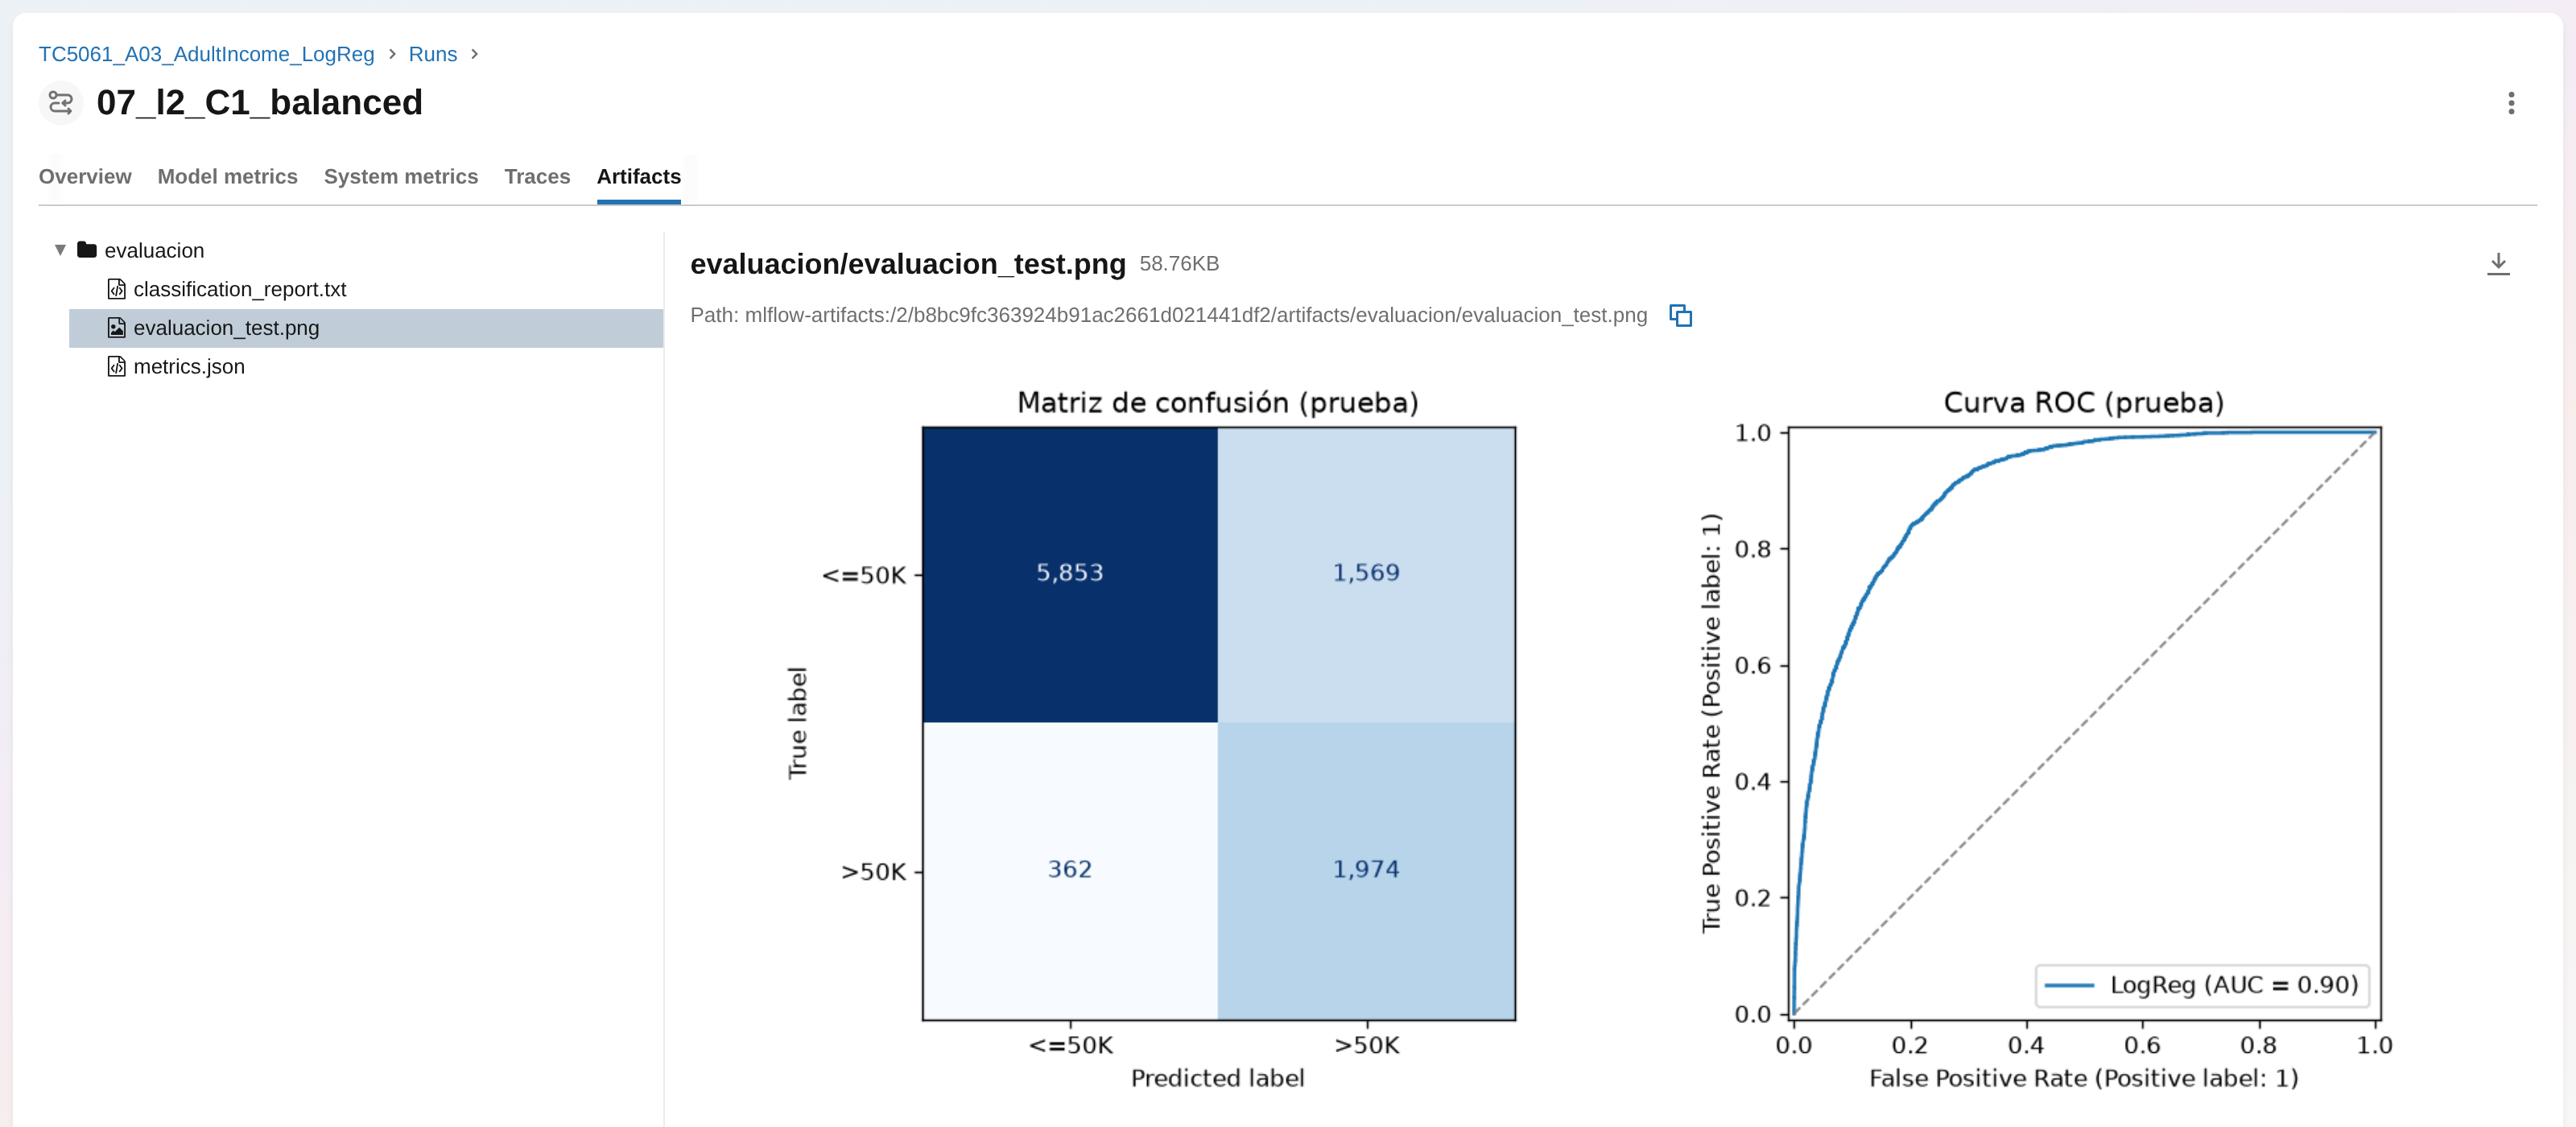
\includegraphics[width=0.9\textwidth]{../evidencia/04_corrida_artefactos.png}
\caption{Artefactos de la corrida \texttt{07\_l2\_C1\_balanced}: reporte, \texttt{metrics.json} y la imagen
con la matriz de confusión y la curva ROC.}
\end{figure}

% ============================== REFERENCIAS ==================================
\newpage
\section*{Referencias}
\sloppy

\noindent\hangindent=1.27cm
Becker, B., \& Kohavi, R. (1996). \textit{Adult} [Dataset]. UCI Machine Learning Repository.
\url{https://doi.org/10.24432/C5XW20}

\noindent\hangindent=1.27cm
Huyen, C. (2022). \textit{Designing machine learning systems: An iterative process for production-ready
applications}. O'Reilly Media.

\noindent\hangindent=1.27cm
Lauchande, N. (2021). \textit{Machine Learning Engineering with MLflow}. Packt Publishing.

\noindent\hangindent=1.27cm
MLflow. (s.f.). \textit{MLflow Tracking} [Documentación]. \url{https://mlflow.org/docs/latest/ml/tracking/}

\noindent\hangindent=1.27cm
Python Software Foundation. (s.f.). \textit{argparse} [Documentación].
\url{https://docs.python.org/3/library/argparse.html}

\end{document}
